\documentclass[12pt,a4paper]{report}

\usepackage[margin=1in]{geometry} % set margin
\usepackage{newtxtext,newtxmath} % set font
\usepackage{titlesec} % customize section title
\usepackage[hidelinks]{hyperref} % enable hyperlinks
\usepackage{graphicx} % read image
\usepackage{longtable} % long table

\setlength{\parindent}{0pt}  % remove paragraph indentation
\setlength{\parskip}{6pt}    % add space between paragraphs

% ==================================================
% Chapter Page
% ==================================================
\newcommand{\chapterpage}[1]{%
    \clearpage
    \phantomsection
    \addcontentsline{toc}{chapter}{\protect\numberline{\thechapter}#1}
    \thispagestyle{empty}

    \vspace*{\fill}
    \begin{center}
        {\fontsize{32}{38}\selectfont\bfseries #1}
    \end{center}
    \vspace*{\fill}

    \clearpage
}

\begin{document}

% ==================================================
% Chapter Heading
% ==================================================
\newcommand{\mychapter}[1]{%
    \noindent
    {\normalfont\bfseries\fontsize{18}{22}\selectfont
    Chapter \thechapter: #1}\par
    \vspace{0pt}
}

% ==================================================
% Section Formatting
% ==================================================
\titleformat{\section}
    {\normalfont\bfseries\fontsize{14}{17}\selectfont}
    {\thesection}
    {0.5em}
    {}

\titlespacing*{\section}
    {0pt}    % left
    {8pt}    % before
    {4pt}    % after

% ==================================================
% CHAPTER 1
% ==================================================
\refstepcounter{chapter}
\chapterpage{Introduction}
\mychapter{Introduction}

\section{Background and Motivation}
\section{Problem Statement}
\section{Research Objectives}
\section{Scope and Limitations}
\section{Significance of the Study}


% ==================================================
% CHAPTER 2
% ==================================================
\refstepcounter{chapter}
\chapterpage{Literature Review}
\mychapter{Literature Review}

\section{Preliminaries}
\section{Relevant Theories and Concepts}
\section{Review of Related Research and Projects}
\section{Identification of Gaps in Existing Solutions}


% ==================================================
% CHAPTER 3
% ==================================================
\refstepcounter{chapter}
\chapterpage{Methodology}
\mychapter{Methodology}

The methodological framework used in this research involves researching, developing, and implementing a hybrid sparse and dense crowd counting system. It explains the overall design of the research, the approach taken for the research, the procedures for obtaining image and video inputs, the analytical methods used during each stage of the research, and the proposed algorithms, models, and techniques that form a major contribution of the system.

\section{Research Design}

This study is conducted using the Design Science Research (DSR) paradigm and an applied, developmental, and experimental (quantitative) research approach. The research problem of obtaining a reliable people count from a single visual sensor across a range of crowd densities is addressed through the design, development, and iterative refinement of a computational artifact, rather than through testing a pre-existing theory. This places the work within the field of engineering and applied computing research, where the creation of a functional and systematically testable system serves as the primary evidence of contribution.

The research design is based on the modular box design for architecture, in which the whole system is divided into a series of independent processing modules. Each stage has a precise computational function, with clearly specified inputs and outputs. The overall research process consists of five iterative steps, as shown in Figure~\ref{fig:research-phases}. This architectural decomposition establishes the system structure before implementation and allows for the development, evaluation, and improvement of individual components of the system. A top-down approach such as this provides an organized framework for experimentation and avoids relying on an ad hoc sequence of computational procedures.

The parameters and configuration settings were arranged in a structured and centralized manner so that different experimental conditions could be varied while keeping other components constant. Therefore, the various stages could be repeated under controlled variations of the parameters. This design is useful because it encourages systematic development, controlled experimentation, and reproducibility, all of which are desirable features of a robust computational research design.

% ==================================================
% RESEARCH DESIGN INFOGRAPHIC
% ==================================================
\begin{figure}[htbp]
    \centering
    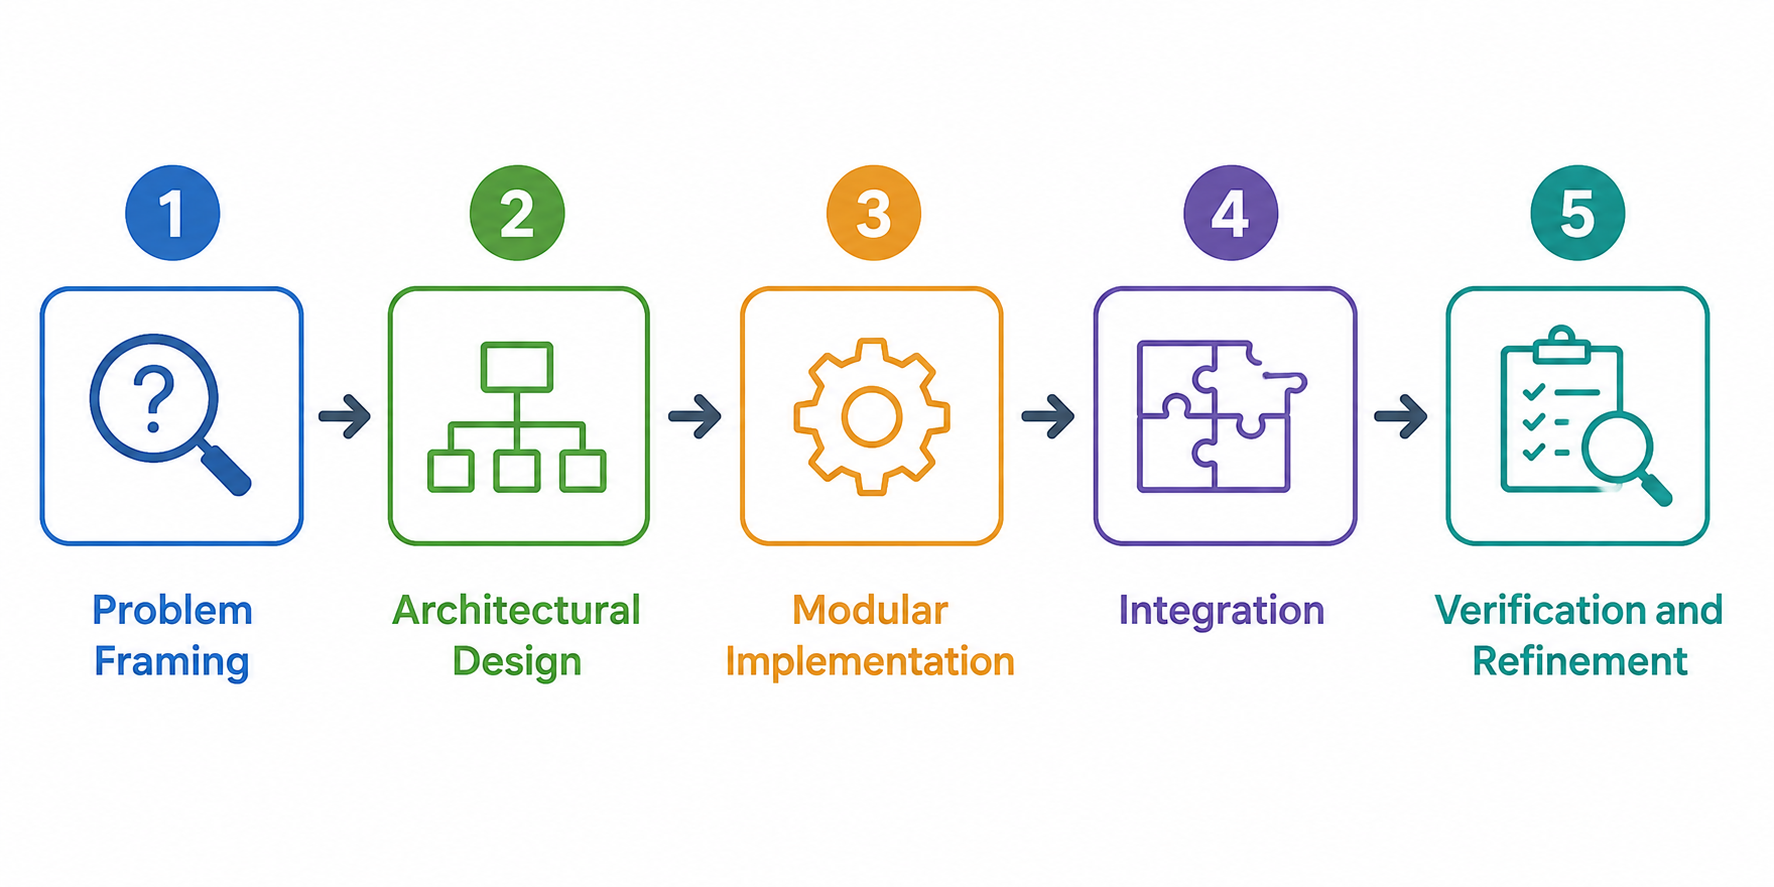
\includegraphics[
        width=0.85\textwidth,
        height=6cm,
        keepaspectratio
    ]{figures/research_phases.png}
    \caption{Research Design Phases}
    \label{fig:research-phases}
\end{figure}

The five phases depicted in Figure~\ref{fig:research-phases} provide a systematic sequence of activities, ranging from problem identification through verification and refinement. The proposed crowd counting methodology is developed and evaluated systematically within each phase.

% ==================================================
% PHASES OF RESEARCH DESIGN
% ==================================================
\begin{longtable}{|p{0.13\textwidth}|p{0.50\textwidth}|p{0.29\textwidth}|}
    \caption{The Phases of the Research Design}
    \label{tab:research-design} \\
    \hline
    Phase & Description & Primary Artifact(s) \\
    \hline
    \endfirsthead

    \hline
    Phase & Description & Primary Artifact(s) \\
    \hline
    \endhead

    \hline
    \multicolumn{3}{r}{\textit{Continued on next page}} \\
    \endfoot

    \hline
    \endlastfoot

    Problem Framing
    &
    Explain the drawbacks and compromises of detection-based methods for
    ``moderately dense'' crowds and regression-based methods for dense crowds,
    and provide the rationale for a hybrid counting framework.
    &
    Problem statement, research objectives, research gap
    \\
    \hline

    Architectural Design
    &
    Break down the proposed system into independent and sequential processing
    steps with distinct inputs, outputs, and responsibilities.
    &
    Pipeline block diagram and system architecture
    \\
    \hline

    Modular Implementation
    &
    Implement individual processing stages as separate computational units
    with well-defined interfaces and structured configuration parameters.
    &
    Individual processing modules and configuration files
    \\
    \hline

    Integration
    &
    Integrate individual components into a single processing pipeline that can
    process the desired visual input modalities.
    &
    Integrated crowd counting pipeline
    \\
    \hline

    Verification
    &
    Execute the integrated system on representative image and video samples;
    examine intermediate system outputs and computational performance;
    detect errors or inconsistencies; and refine parameters and processing
    strategies relevant to the integrated system and its execution.
    &
    Experimental results, validation outputs, and refined configurations
    \\
    \hline

\end{longtable}

This design is not only experimental but also non-descriptive. The pipeline
includes toggleable backends, such as YOLO-based detection and Haar-cascade
detection, as well as classical density estimation and neural density
estimation. These alternatives enable the comparison of different processing
backends using the same input data. Consequently, the research involves a
series of controlled experiments rather than evaluation of a single fixed
system configuration.

\section{Research Approach}
\section{Data Collection Methods}
\section{Data Analysis Techniques}
\section{Proposed Algorithm/Model/Techniques}


% ==================================================
% CHAPTER 4
% ==================================================
\refstepcounter{chapter}
\chapterpage{Requirements Analysis and Specification}
\mychapter{Requirements Analysis and Specification}

\section{Elicitation and Documentation of Requirements}
\section{Functional Requirements}
\section{Non-functional Requirements}
\section{Use Cases and Scenarios}


% ==================================================
% CHAPTER 5
% ==================================================
\refstepcounter{chapter}
\chapterpage{System Design and Architecture}
\mychapter{System Design and Architecture}

\section{System Architecture Overview}
\section{High-Level Design}
\section{Detailed Design}
\section{Component and Module Design}
\section{Database Design}


% ==================================================
% CHAPTER 6
% ==================================================
\refstepcounter{chapter}
\chapterpage{Implementation and Development}
\mychapter{Implementation and Development}

\section{Programming Languages and Technologies Used}
\section{Implementation Details}
\section{Testing and Debugging Approaches}
\section{Version Control and Configuration Management}


% ==================================================
% CHAPTER 7
% ==================================================
\refstepcounter{chapter}
\chapterpage{Results Analysis and Discussion}
\mychapter{Results Analysis and Discussion}

\section{Data Collection and Analysis}
\section{Evaluation Metrics and Criteria}
\section{Interpretation of Results}
\section{Comparison with Related Work}
\section{Discussion of Findings}


% ==================================================
% CHAPTER 8
% ==================================================
\refstepcounter{chapter}
\chapterpage{Conclusion and Future Work}
\mychapter{Conclusion and Future Work}

\section{Summary of Contributions}
\section{Limitations and Challenges}
\section{Recommendations for Future Enhancements}


% ==================================================
% References
% ==================================================
\newpage
\renewcommand{\bibname}{References}
\bibliographystyle{IEEEtran}
\bibliography{references}

\end{document}